\documentclass[12pt,a4paper]{report}
\usepackage[utf8]{inputenc}
\usepackage[T1]{fontenc}
\usepackage[francais]{babel}
\usepackage{a4wide}
\usepackage{graphicx} 
\usepackage{cmbright}
\usepackage{fancyhdr}
\usepackage{url}
\usepackage{shorttoc}
\usepackage{listings}
\usepackage{framed}%, mdframed}
\usepackage{xcolor}
\usepackage{moreverb}
\usepackage[body={16cm,25cm}]{geometry}
\DeclareGraphicsExtensions{.pdf,.eps,.eps,.jpg,.mps} 
\pagestyle{fancy}
\fancyhead[LO]{Projet SR II}
\fancyhead[RE]{\rightmark}
\fancyhead[RO,LE]{\thepage}
\fancyfoot[CO]{\hrule\smallskip B. Bezançon - C. Molin}
\fancyfoot[CE]{\hrule\smallskip Master 1 - Informatique - 2013/2014}


\renewcommand{\thesection}{\arabic{section}}

\begin{document}

\begin{titlepage}
	\begin{center}

	\vspace*{4cm}
	\hrule\bigskip
	
	{\LARGE\bf Projet de cryptographie}
	\bigskip

	{\normalsize Master 1 - Informatique -- 2012/2013}
	\bigskip
	\hrule
	\vspace*{2cm}

	\vspace*{5cm}

	Benjamin Bezançon - Charles Molin
	\end{center}
\end{titlepage}
\shorttableofcontents{Sommaire}{1}
%\listoffigures
	
	\newpage
	\chapter*{Introduction}
	\addcontentsline{toc}{chapter}{Introduction}
	
	\newpage
	\chapter*{Codage de Huffman}
	\addcontentsline{toc}{chapter}{Codage de Huffman}
	En 1952, David Huffman a élboré un algorithme de compression sans perte. C'est une méthode statistique qui permet d'attribuer un mot de code binaire aux différents symboles à compresser. Dans la suite de cette partie nous allons expliquer la mise en oeuvre de cette algorithme dans notre projet. \\\\
	La première étape est la création d'une table de fréquence, pour chaque caractère présent dans la chaîne à coder nous lui associons une fréquence d'apparition.\\\\ Prenons l'exemple avec le mot TEXTE, voici la table que nous obtenons:\newline
	\begin{center}
	\begin{tabular}{|c|c|}
		\hline
		Clé & Fréquence\\
		\hline
		'X' & 1 \\
		'E' & 2 \\
		'T' & 2 \\
		\hline
	\end{tabular}
	\end{center}
	Dans la deuxième étape nous réalisons un arbre binaire composé de noeud. \\
	Etape 1: On créer un noeud terminal pour chaque ligne du tableau.
	\begin{center}
	\begin{figure}[!h]
	\centering
	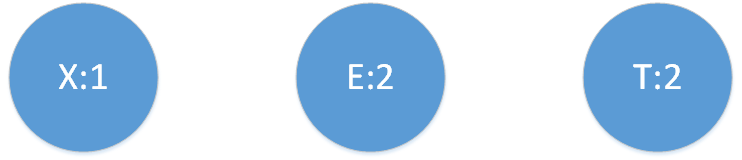
\includegraphics[width=0.40\textwidth]{etape1.png}
	\caption{Etape 1}
	\end{figure}
	\end{center}
	Etape 2: On supprime les deux arbres ayant la plus petite fréquence on les remplace par un "arbre somme". On reproduit cette étape jusqu'à ce qu'il nous reste plus qu'un seul arbre. 
	\begin{center}
	\begin{figure}[!h]
	\centering
	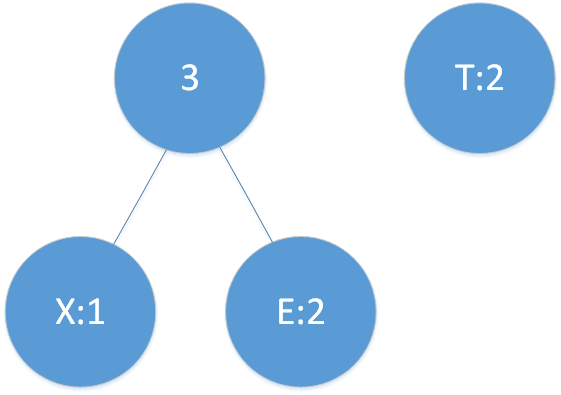
\includegraphics[width=0.30\textwidth]{etape2.png}
	\caption{Etape 2}
	\end{figure}
	\end{center}
	Etape 3: L'arbre final
	\begin{center}
	\begin{figure}[!h]
	\centering
	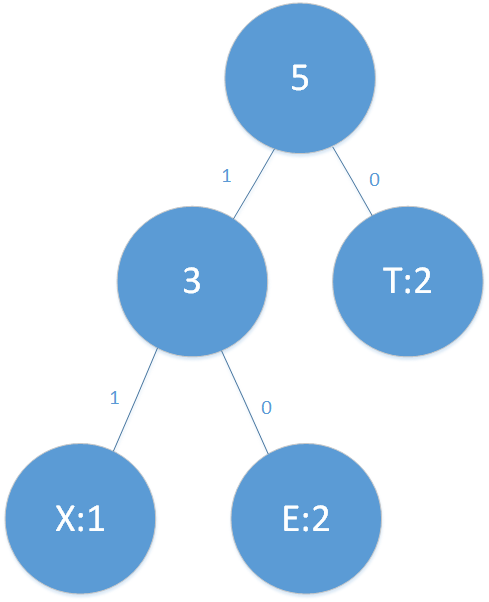
\includegraphics[width=0.30\textwidth]{etape3.png}
	\caption{Etape 3}
	\end{figure}
	\end{center}
	Ensuite pour obtenir le code binaire, on parcourt l'arbre en partant de la racine jusqu'au noeud terminal et on obtient le tableau suivant:\\
	\begin{center}
	\begin{tabular}{|c|c|}
		\hline
		Clé & Code binaire\\
		\hline
		'X' & 11 \\
		'E' & 10 \\
		'T' & 0\\
		\hline
	\end{tabular}
	\end{center}
	Voici le mot TEXTE, transcrit avec notre nouveau code:\\
	01011010\\\\
	Maintenant nous allons calculer le taux de compression. Le mot TEXTE contient 5 caractères codés sur 8 bits ce qui resprésente 40 bits et le nouveau codage contient 8 bits. On obtient donc un taux de compression de 80\%.

	\chapter*{Conclusion}
	
	\addcontentsline{toc}{chapter}{Conclusion}
\setcounter{tocdepth}{2}
\end{document}

